\chapter{Process Management and Scheduling}
\label{chap:ProcMngtSchedMain}

Data is coming in at different, independent rate from sensors and is produced asynchronously from internal processing elements.
For certain processes, processing the incoming data as quickly as possible is key, however, this is challenging for several reasons:
1) a process may subscribe to multiple, independent streams with asychronized report schedules and 2) interpolated values
should be avoided to minimize prediction inaccuracies in interpolated values.  Therefore, a process actually wants all the freshest
data from all the streams they are subscribing to, while minimizing the average time that the data for each respective stream has 
been waiting in the buffer.

Sensor data is fundamentally challenging to deal with because much of it must be cleaned before it can be processed.  For example,
it is not uncommon to receive readings that is out of operational range, that is erroneous with respect to the previous observed trend,
or to stop receiving readings altogether.  This implies the need for processing jobs to provide a level of filtering over the raw streams.
Once the data is cleaned, it is typically consumed more sophisticated processes that aggregate the information or use it for control
of the space or equipment.  We provide the mechanisms for handling both classes of processing jobs with our process management layer.
In the next section we will discuss our process management layer and how users can both submit jobs to StreamFS for management or link
their own external processing elements so that they can be managed through StreamFS but run outside of StreamFS.

% \input{ProcessMngt}
\section{Internal Processes}
\label{sec:internalprocs}

Internal processing jobs are short jobs submitted by users that are managed by StreamFS.  When a user submits
a job they specify the name of the job in the request.  The process definition is checked for syntax correcteness
and if it is okay, then it is accepted.  All newly created job definitions are placed in \texttt{/proc}.


\begin{lstlisting}[caption={Simple aggregator process job.},label={code:simple_agg}]
function(buffer, state){ 
    var outObj = new Object();
    var pavg = state.cnt;
    var sum =0;
    for(i=0; i<buffer.length; i++){
        sum += buffer[i].value;
        state.cnt+=1;
    }
    outObj.value = sum;
    state.avg = (state.avg * pavg + sum)/state.cnt;
    return outObj;
}
\end{lstlisting}


The code in Listing~\ref{code:simple_agg} gives an snippet of example code that aggregate the data 
passed to it in the buffer.  If the user names this definition \texttt{simpleagg}, then the file that corresponds to 
the job definition is \texttt{/proc/simpleagg}.  We do not check the size and complexity of the job, however, we
strongly recommend that jobs be kept small and simple.  Generally, we recommend that a job pipeline 
be established rather than feeding one large chunk of code.  It makes the pipeline easier to debug once it is
activated.

In order to activate the process, the user must pick a set of streams and initiate a subscription \emph{pipe}.  The 
\emph{subscription manager} notes that the sink in a process definition file and informs the \emph{process manager}.
The process manager fetches the code and passes it to a node in the processes cluster.  The process manager
generates an id and passes it back to the subscription manager.  That code is used as a new \emph{instance file} that 
represents the output of the file and that instance file is created in the process file definition file's folder.
So if the id generated is \texttt{550e8400} the corresponding file is \texttt{/proc/simpleagg/550e8400}.
This file instance is a stream file (which we discuss is detail in chapter~\ref{chap:naming}), which allows the user
to pipe it to another sink.  There is also some metadata information that is associated with each of the files created.
The instance file contains information about the streams it is consuming and various statistics, such as 
execution time and execution period.  If the user deletes the file the subscription is deleted and the process manager sends
a kill message to the corresponding process element.

The function must have the signature as shown above, where the first parameter is the \texttt{buffer} and the second parameter
is a \texttt{state} variable.  It must also return a variable of type \emph{object}.  The \texttt{buffer} is an array of \texttt{data}
objects.  Each \texttt{data} object contains two fields, a \texttt{ts} field that is the timestamp
for the data point and the \texttt{value} field which is the value for the data point.  An optional setting is to also
include all attribute-value pair values that are part of the metadata associated with the corresponding stream file for the stream.
The \texttt{state} variable is an object that is passed across executions of the function.  This way the function could maintain
any necessary state without losing it after a single run of the job.  Upon creation, the user specifies other parameters that
drive the execution period and/or execution conditions for the job.  The user specifies the \texttt{window} size and/or a
\texttt{timeout} parameter.  If the \texttt{window} is of size $k$ then the job will run when the incoming buffer for the job has
at least $k$ elements in it.  The \texttt{timeout} sets the minimum period for the job to run.  If both are specified the 
\texttt{timeout} always runs and the job will also run when/if the buffer has at least $k$ elements.

\subsection{Process Element}

\begin{figure}[th!] %htbp
\centering
\includegraphics[width=0.85\columnwidth]{figs/pe_internals}
\caption{This figure shows the internal structure of a process element (PE).  The PE consists of several
javascript sandboxes where internal process code runs.  It also contains a scheduling loop, message router, and instance 
monitor.}
\label{fig:pe_internals}
\end{figure}


The process element stub that runs on a separate machine.  Its main job is to manage the jobs that are being executed on that
machine.  Figure~\ref{fig:pe_internals} shows the components of a process element.  There are four main components in the unit.

\begin{enumerate}
\item \emph{Scheduler}: The scheduler manages the execution schedule for each job running in a sandbox.  The scheduler uses
the \texttt{timeout} as the execution period of the job.

\item \emph{Sandbox}:  The sandbox is where the javascript code runs.  The sandbox contains an input and output buffer and simply 
waits for either an execution signal from the scheduler or until the input buffer has \texttt{window} element in it.  The output
buffer is of size 1.  The object returned by the job is written to the output buffer.

\item \emph{Message Router}:  The message router communicates with the process manager and sends control and data messages between
the PE and the process manager.  It monitors the output buffer for each of the elements and forwards them to the process manager 
when it is populated.

\item \emph{Instance Monitor}:  The instance monitor manages the state of the sandbox.  If a sandbox dies, the instance monitor re-starts
it.  If it continues to die, it kills the sandbox process and forwards an error message to the message handler to the process manager.
The process manager annotates the instance file with the error.

\end{enumerate}


The process manager keeps a map of which process elements own which jobs.  If a process element goes down, the jobs are automatically
migrated to another process element and the process element is removed from the active list.  Each PE and job have a unique identifier.
The messages received from the \emph{message router} in the PE are annotated with these ids and the process manager uses these
to update the associated instance file in StreamFS.  Again, everything is managed in through filesystem.  So errors and data
are exposed to external applications through the meta/data in the files.

Note, the process manager maintains a mapping between job instances and PEs.  It also notes the machine the PE is running on.  The
\emph{instance monitor} allows the process manager to make decisions about job migration in case of failure.  PEs are designed
to function independently from one another.  This allows the process cluster to scale linearly with the load -- in terms of
the number of streams being processed and the number of active jobs.  Like the other components in StreamFS, it is 
\emph{horizontally scalable}.  The process manager serves as a single point of failure.  If it fails it must be restarted manually.
Any messages sent from the PE to the process manager during the down period is lost.

% Our contributions are:  

% \begin{itemize}
% \item Use of the entity-relationship graph to provide OLAP \emph{roll-up}, \emph{drill-down},
%         and \emph{slice and dice} operations.
% \item Show how sliding-window operations can be used on real-time data in combination with the entity-relationship
%         graph to maintain accurate aggregates as the underlying objects and inter-relationships change.
% \end{itemize}

% \subsection{Mapping OLAP to ERG}
\subsection{OLAP-style Aggregation}

% \begin{itemize}
% \item Introduction to OLAP.
% \item Explanation of ERG in StreamFS.
% \end{itemize}
Online analytical processing (OLAP) provides summarization of data
from a set of underlying data repository (date warehouses).  Traditionally, OLAP is used to process
business data.  Business data summarization allows an analyst to ask targeted questions about aggregates 
and trends in their data.  The data is typically multidimensional in nature and operations can be performed with
respect to those dimensions and their inter-relationship.  In our deployments, we find that most queries are 
similar to OLAP queries with scan-heavy queries across the time dimension.

We introduce a mechanism that can perform hierarchical aggregates across a unit of measure, used in combination
with the timeseries data store to support scan-heavy queries, called \emph{aggregation points}.  We discuss
these in more detail in section~\ref{sec:aggpts}.  However, before discussing aggregation points, we give details
on how we make use of the entity-relationship graph and timeseries database to support OLAP-style queries.

OLAP schemas logically construct a hypercube with different dimensions along each axis.  We presented a visual translation of
a OLAP cube to an entity relationship graph in section~\ref{sec:erg2olap}.  Specifically, we showed in Figure~\ref{fig:olap2erg}
that each dimension is essentially a unit of measure, the hiearchy is explicitly constructed, and there
time is a dimension that is stored in a timeseries database.  We show how the terminology also translates and some
examples of certain classes of OLAP queries, how they are constructed, and how they are satisfied by StreamFS.

\subsubsection{Measures, Dimenions, and Levels}
\emph{Measures} refer to the actual value, located somewhere is the cube along the intersection of several dimensions.
A \emph{dimension} is simply a reading and an example is shown in Figure~\ref{fig:olap2erg}.  Dimensions 
are labels for an axis.  In StreamFS a measure is a unit of measure (i.e. Fahrenheit) or time.  The hierarchical \emph{level}
is explicit in the construction of the names.  So in the subtree that organizes streams according to the location of the
in space, the floor level would be above the room level.  These points can be designated as aggregation points, whereby
all streams that have the specified units, are aggregated at that point and the data are stored like any other streams.

\subsubsection{Operations: drill-down and roll-up}
Drill-down and roll-up are explicit in the structure.  You can drill down to individual readings or roll them
up into an aggregation point at a particular level in the hierarchy.  Essentially the level is an explicitly specified in the 
name of either the raw stream or the aggregation point.

\subsubsection{Operations: Slice and Dice}
Slice and dice queries are queries that either take a slice of the cube along a dimension or pick a sub-cube from the cube.
Slice and dice operations are translated as traversals of the hierarchical structure across levels and units.  Figure~\ref{fig:olapslice2ergslice}
shows how a slice query is satisfied on a hierarchical structure.  The corresponding slice query 
is \texttt{query.slice('/4F/R*').start(t1).end(t2);}.

\begin{figure}[h!] %htbp
\centering
\includegraphics[width=1.0\columnwidth]{figs/olapslice2ergslice}
\caption{This figure shows how a ``slice'' operation is translated from the cube to the ERG.  The user queries across all streams or aggregation
points at a certain level, specified by a star level query with the level-specific prefix.  The corresponding slice query is
\texttt{query.slice('/4F/R*').start(t1).end(t2)}.
}
\label{fig:olapslice2ergslice}
\end{figure}


% \begin{lstlisting}[caption={Slice query example.},label={code:slice_query}]
% query.slice('/4F/R*').start(t1).end(t2);
% \end{lstlisting}

Figure~\ref{fig:olapdice2ergdice}
shows how a dice query is satisfied on a hierarchical structure.  The corresponding dice query 
is \texttt{query.dice('/4F/R*').units(['F']).start(t1).end();}.


\begin{figure}[h!] %htbp
\centering
\includegraphics[width=1.0\columnwidth]{figs/olapdice2ergdice}
\caption{This figure shows how a ``dice'' operation is translated from the cube to the ERG.  The user queries across all streams or aggregation
points at a certain level, specified by a star level query with the level-specific prefix.  The corresponding dice query is
\texttt{query.dice('/4F/R*').units(['F']).start(t1).end()}.}
\label{fig:olapdice2ergdice}
\end{figure}


% \begin{lstlisting}[caption={Dice query example.},label={code:dice_query}]
% query.dice('/4F/R*').units(['F']).start(t1).end();
% \end{lstlisting}


\subsubsection{Operations: Pivot}
Pivot operations are not explicitly supported.  Although you can imagine that if you cut across a hierarchical level across all dimension, can
can effectively construct a pivot-style query.



\subsection{Aggregation Points}
\label{sec:aggpts}
StreamFS makes use of OLAP-style mechanism to provide the end-user with \emph{aggregation points} in the hierarchy.
StreamFS distinguishes between nodes that represent streaming data sources and those that do not.  Those that do not, 
however, can be tagged as aggregation points.  
% As part of the tagging processes, a user specifies the units of aggregation, with 
% additional options for cleaning and processing.  
When node is tagged as an aggregation point all the points root at that
node in the tree are set as aggregation points and all streams are aggregated and save to the timeseries database.
Since streams are not synchronized (i.e. they do not produce data at the same time) each time a value arrives from a
sensor the value for all other streams is interpolated and aggregated along the \emph{unit} level dimension.
%an example?

This propagates up to the aggregation point and all of it is saved in the timeseries database.  The aggregation function
can be specified by the user, with the default set to as \texttt{sum}.  Other options include \emph{avg, sum, max, min} and
a custom function that can be specified by the user. %pointer to an internal/external process definition file
% Aggregation points are also critical for support OLAP-style queries and \emph{dynamic aggregation}, discussed in
% the next two sections.

%FILL IN WITH REAL GRAPH
\begin{figure}[htb!]
\begin{center}
\includegraphics[scale=0.6]{figs/aggtree}
\caption{This shows an illustration of the aggregation tree used by \emph{dynamic aggregation}.  Data flows from 
the leaves to the root through user-specified aggregation points.  When the local buffer is full the streams
are separated by source, interpolated, and summed.  The aggregated signal is forward up the tree.}
\label{fig:aggtree}
\end{center}
\end{figure}

% Aggregation points combine the underlying entity-relationship graph with in-network aggregation.  It treats
% each node in the graph as a potential point of aggregation on a particular data type.  
Consider the following example.  We need to compute aggregates of \emph{KW} data and we declare the node for a particular room as
the point of aggregation, we accept data from all children of that node that, whose units are in \emph{KW},
and add the streams together over pre-defined window size or pre-defined timeouts.

The scheme is hierarchical, so a node only accepts data from its children and only sends data to its parent.
StreamFS checks for cycles when before node insertion and prevents double-counting errors by only allowing 
aggregation-points that are roots of a tree that is a sub-graph of the entity-relationship graph.  In our deployment,
each view is a managed as an independent hierarchy.  So the hierarchy of \emph{spaces} is separate from
the \emph{inventory} hierarchy or the \emph{taxonomy} hierarchy.  This allows us to ask questions with a particular
view in mind, without conflict, and is a natural fit for our aggregation scheme.

% \subsubsection{How it works}
Although there are different semantics applied to different file types at the application layer, dynamic aggregation
mainly deals with two types of files: (1) container nodes and (2) stream nodes.  The main difference is that \emph{container} nodes
are not explicitly associated with data coming from a sensor and \emph{stream} nodes are.  Furthermore, container
nodes can have children, while stream nodes cannot.  In our application, meters are represented by container nodes
and each stream of data they produce is a stream node.

When an aggregation point is enabled, dynamic aggregation places a buffer at the node for the type
of data that should be aggregated.  
If we want to aggregate \emph{KW} data, we specify the type and send an enable-aggregation
request to StreamFS.
% to the node through an HTTP {\texttt POST} to the path for that node.  
The flow of data starts at the leaves when
a stream node receives data from a sensor.% through HTTP {\texttt POST}.  
As data arrives it is immediately
forwarded upstream to the parent(s).  
% If a node that receives data from its children is an aggregation point it buffers
% the data, otherwise it forwards it to its parent.

Ignoring the timeouts for now, lets imagine the parent is a point of aggregation and its buffer is full.  At this point
the parent separates data into bins for each source and cleans it for aggregation through interpolation.  The main
operation is to \emph{stretch} and \emph{fill} that data with linearly interpolated values.  The \emph{stretch}
operation orders all the timestamps in increasing order and, for each bin, interpolates the values using the
first (last) pair of data points.  If there is only a single data point, the stretch uses it as the missing value.
The \emph{fill} operation find the nearest timestamps that are less-than and greater-than the missing sampling time, 
uses their values to determine the equation of a line between them and interpolates the missing value using that equation.
Once this is done for each signal, the values are added together for each unique timestamp and the aggregated
signal is reported to the parent, where the operation occurs recursively to the root.
Figure~\ref{fig:aggtree} shows an illustration of this processing structure.


% \subsection{Dynamic Aggregation}


%problem:  the buffer size has to increase exponentially up the tree, in order to not drop any values.
%solution: chuck the data into default-buffer sized pieces and parallelize the interpolation using the interpolated tasks technique




\subsubsection{Dealing with dynamics}
\label{sec:dynagg}

This approach deals with changes in the graph quite naturally.  All aggregation points deal only with local data, so
a node is only concerned about the children that give it data and the parent to send data to.  As objects in the environment
move from place to place and these changes are captured, the entity-relationship graph also changes to reflect the move.
This change in aggregation constituents is naturally accounted for in the aggregate.  Since the underlying pub-sub mechanism
drives the forwarding (see Section~\ref{sec:ProcMngtSchedMain}) the removal of a child will reject any new data that comes 
in for the removed node.  As such, it will
not be accounted for in the aggregate.  If a new child is added, it is forwarded up the tree, since the name associated
with the data point will indicate its position in the hierarchy.
% When a child is removed,
% it no longer forwards data to the old parent, therefore the aggregate will reflect that change.
Note, however, that changes in the entity-relationship graph are indistinguishable from energy-consuming items that have
been turned off.  For the purposes of aggregation, that is okay.

OLAP-style aggregation is an expensive feature.  Each point in the subtree rooted at the aggregation point is automatically
activated to produce streaming data.  Special internal processing elements are enabled to compute the aggregates and run
the pre-processing and communication between the processing unit and name server increases as data is returned from the 
process elements to be routed to the timeseries data store.  The amount of processing and storage scales linearly with the 
number of streams and the number of aggregation points in the sub-tree.



% For demonstration lets have the user turn off on of their appliances when they leave as well.  This should cause that total
% room aggregate to drop, the person's personal aggregate to drop, but the other occupant's aggregate to remain
% the same.

% %FILL IN WITH REAL GRAPH
% \begin{figure}[htb!]
% \begin{center}
% \includegraphics[scale=0.39]{figs/blankbox}
% \caption{A room with items that belong to many users.  Person leaves with their item, aggregate falls.  Show aggregate.
% Person joins another room, aggregate in that room rises.  Show aggregate in the new room.  Compare before and after.}
% \label{fig:personaltotalagg}
% \end{center}
% \end{figure}

% Figure~\ref{fig:personaltotalagg} illustrate the results of the second scenario.  Note how...


\section{External Processes}
\label{sec:externalprocs}

% External processing jobs can be centrally managed in StreamFS as well.  
In real deployments, %it is often the case that
users do want to be limited by the particular libraries that are available to them in javascript or they have already made
a signficant investment in time writing and testing their own processing jobs.  For them, we provide an external client stub that 
re-directs data from standard in/out through a network connection to/from the StreamFS process manager.  The stub also interprets
process management commands to spawn and kill jobs and associate different subscriptions with different instances of a jobs 
running on the client side.

\begin{figure}[h!] %htbp
\centering
\includegraphics[width=0.55\columnwidth]{figs/external_stub}
\caption{External process stub.  Note, it contains similar component to a process element and functions much the same way, 
managing the buffers, scheduling, errors, and communication on the client side like the PE.}
\label{fig:external_stub}
\end{figure}

Figure~\ref{fig:external_stub} shows the internal components of a client stub.  Note, it contains very similar components to
a process element and work in a similar fashion.  The client stub contains the four major components:

\begin{enumerate}
\item \emph{Scheduler}: The scheduler schedules the execution of jobs on the client machine.  It uses the \texttt{window} and
						\texttt{timeout} parameters to set when and how often the job is set to run.
\item \emph{Process}:  The process component is simply in charge of managing communication with the process that is spawn
						on the local machine.  It maintains an pipe to each local process.  The processes
						run indepdently and share no memory directly.  Data from the input buffer is copied to the 
						pipe connection to the process.
\item \emph{Message Router}: The message router maintains a socket connection to the Process Manager and writes to the associated
								buffer for specific jobs.
\item \emph{Instance Monitor}: The instance monitor re-starts jobs when/if they fail and forward local errors to the process manager
								to annotate the associated files in StreamFS.
\end{enumerate}

On startup, the client stub read a local configuration file that specifies the path to the job and metadata that describes
job.  These are used to register the job with StreamFS and set the metadata attributes.  The registration on the StreamFS 
server is exposed through an \emph{external process} file.  The user interact with an external job exactly the same way they
interact with an internal process job.  In order to spawn a job on the client, the user simply ``pipes'' a stream file 
to the external process file.  The creation of the pipe/subcription send a spawn message to the client and starts the associated
job on the client.  Once the process is started, data from the stream(s) is forwarded to the client, which writes it to the 
standard-in of the client job.  Starting a job also creates a stream file the StreamFS server.  Any data that's produced by the job
and written to standard-out is re-directed to the server and made available through the stream file.

This desgin is consistent with the semantics of pipe/subscription management and functionality.  Recall, internal processes
work the same way and this allow us to stay consistent with the file-centric principal whereby \emph{everything is managed
through the filesystem itself as a file}.



\section{Maximizing Data Freshness}
\label{sec:freshness}

Data is coming in at different, independent rate from sensors and is produced asynchronously from internal processing elements.
For certain processes, processing the incoming data as quickly as possible is key, however, this is challenging for several reasons:
1) a process may subscribe to multiple, independent streams with asychronized report schedules and 2) interpolated values
should be avoided to minimize prediction inaccuracies in interpolated values.  Therefore, a process actually wants all the freshest
data from all the streams they are subscribing to, while minimizing the average time that the data for each respective stream has 
been waiting in the buffer.

Certain jobs only care about consuming the latest readings from their subscription streams.  They are willing to discard reading until two
conditions are met:

\begin{enumerate}
\item There is at least one data point from each stream in the subscription buffer.
\item The statelness factor is minimized within the immediate time window.
\end{enumerate}

This is of particular interest to controllers that need to make control decision based on the freshest data possible and can tolerate some variability
in the completion time of the control task.  It is also useful in analytical jobs that want to process the latest data from multiple streams while also
allowing some variability in the completion of the processing task.  Note, there's a fundamental tradeoff
between the staleness factor and variability of consumption.  It is sometimes better to wait for the next incoming data point than it is to use what
is currently in the buffer, as waiting will decrease the overall staleness factor.  Other times, it is better to consume the bufferred data immedaitely.
This causes a certain amount of variability in the delivery period to the control process.  However, for some applications, this is a reasonable tradeoff
to make.  Making use of the freshest data is desirable for minimizing errors, either in the control of a system or the calculation of some aggregate state.
Generally, the error grows with staleness, therefore the goal of this mechanism is to continuously minimize the error associated with staleness through
scheduling.


\begin{figure}[t!] %htbp
\centering
\includegraphics[width=0.75\columnwidth]{figs/min_buffer}
\caption{Multiple streams in a subscription and their associated parameters.}
\label{fig:min_buffer}
\end{figure}

Let $A_{i}$ be the arrival time of the last data point received from stream $i$ and $D_{i}$ be the arrival time for the next data point from stream $i$
and their relationship as described in equation \ref{eqn:deadline}, where $T(i)$ is the average period between the arrivals from stream $i$.

\begin{equation}
D_{i} = A_{i} + T(i)
\label{eqn:deadline}
\end{equation}


Periodically, our algorithm runs and checks if there is a data point for each stream in the subscription.  If so, the \emph{min\_buffer} algorithm runs 
and effectively decides whether to execute the job on the current buffer immediately or whether to wait until later, when the \emph{staleness factor} of
the buffer will be at a minimum.  This decision is driven by equation~\ref{eqn:later_better_condition}, whereby we find the next deadline, computed with
equation~\ref{eqn:last_deadline}, for each stream in the set and determine the staleness factor will be for the entire buffer if we wait until that deadline arrives.

\begin{equation}
t_{L,i} = A_{i} + \Bigl\lfloor \frac{D_{k}-A_{i}}{T(i)} \Bigr\rfloor T(i)
\label{eqn:last_deadline}
\end{equation}

If there is no deadline $D_{k}$ for some stream $k$ such that equation~\ref{eqn:later_better_condition} holds, then we execute now.  Otherwise we choose to wait
until $D_{k}$ for the stream whose next deadline minimizes the staleness factor of the buffer.


\begin{equation}
\sum_{i=1}^{k-1} D_{k} - t_{L,i} < \sum_{i=1}^{k} t_{now} - A_{i}
\label{eqn:later_better_condition}
\end{equation}

The algorithm is sketched our below.


\begin{algorithm}[h!]
 \SetAlgoLined
 Given a full buffer $b[n]$:\\
  \For{all elements in the $b$}{
  (1) Calculate the staleness of element $i$ and add to total stalness, $S_n$\;
  \For{all other elements in the buffer}{
  	(1) Determine the next report time $D_i$ for this element\;
  	(2) Determine the staleness of all the elements if we wait until $D_i$\;
  	(3) If it is the smallest staleness figure calculate, replace minimum cost, $S_l$.
  	}
  }
  \If{$S_l$ is less than $S_n$}{
  (1) Wait until later to consume\;
  \Else{
  (1) Consume now}
  }
 \caption{\texttt{min\_buffer} algorithm.}
 \label{alg:emd}
\end{algorithm}


\section{Results}
This section emphasize the advantages of EMD to efectively uncover correlated signals/sensors(?).
First, we demonstrate the benefit of EMD with a simple example, the three sensorsr presented in Section \ref{problem}.
Second, we validate the proposed methodology with a large dataset (674 sensors) and highlight that EMD uncovers the spatial correlation of the sensors.

\begin{table*}
\begin{center}
\begin{tabular}{|l|l|l|l|l|l|}
\hline
× & Raw signal & 1st IMF & 2nd IMF & 3rd IMF & Residual\\ \hline
EHP, Light & 0.7720 & 0.4431 & 0.5104 & 0.6171 & 0.8114\\ \hline
EHP, GHP & 0.6369 & -0.0055 & 0.0883 & 0.2350 & 0.7956\\ \hline
\end{tabular}
\caption{Correlation coefficients of the analyzed signal and their IMFs uncovered by EMD}
\label{tab:corr}
\end{center}
\end{table*}
\subsection{Simple Scenario}

Lets consider the simple example of Section \ref{problem} where we would like to know if an EHP signal is correlated with the two other signals; a light signal and a GHP signal.
Using the raw signals, the correlation coefficients suggest that the light and GHP signals are both correlated to the EHP signal (Table \ref{tab:corr}).
As stated in previous section this result is certainly biased by the strong daily pattern shared by these three signals.

Extracting the weekly pattern of the data using EMD permits a more detailed analysis of these signals.
Figure \ref{fig:emd} depicts the EMD decomposition of the three signals.
Notice that the EMD process has been stopped once the daily pattern have been uncovered.
Thereby, for each signal EMD has retrieved three IMFs that highlight the high frequency characteristics of the signals.

The correlation coefficients for the EHP and light IMFs --- i.e. $0.4431$, $0.5104$ and $0.6171$ corresponding respectively to the IMF1, IMF2 and IMF3 --- emphasize the positive correlation of the two signals in the high frequency domain.
However, the correlation coefficients for the EHP and GHP IMFs show that the two signals are independent in the high frequency domain.
Therefore, EMD allow us to effectively identify that the light signal is related to the EHP whereas the GHP one is not.

\begin{figure*}
\centering
 \subfigure[Raw signals correlation coefficients]{\label{fig:histo1}\includegraphics[width=.45\textwidth]{img/allFloors_week1_week4_corr_abs.eps}}
 \subfigure[Average IMFs correlation coefficients]{\label{fig:histo2}\includegraphics[width=.45\textwidth]{img/allFloors_week1_week4_emd_abs.eps}}
 \caption{Distribution of the correlation coefficients of the raw signals and corresponding IMFs using 3 weeks of data from 674 sensors deployed on 12 Floors.}
\label{fig:histo}
\end{figure*}

\subsection{Validation}


In order to validate the effectiveness of the proposed approach to identify correlated signals, we analyze three week signals from the 674 sensors deployed in the building.
For each signal $S$ we compute the correlation coefficient for $S$ and the EHP signal and the average value of the IMFs correlation coefficients obtained with EMD.
Figure \ref{fig:histo1} shows the distribution of the raw signal correlation coefficients.
Regarding this figure a large fraction of the dataset seems to be correlated with the EHP signal.
Indeed half of the analyzed signals provide a correlation coefficient higher than $0.36$.
Although the highest score correspond to the light signal that is actually from the same room as the EHP signal, all signals that achieve a score higher than $0.6$  correspond to 118 heat pumps that are located at different floors and are independent from the analyzed EHP signal.
Moreover, the distribution of the signals is almost uniform, thus, discriminating signals correlated to the analyzed one is a laborious task.

Figure \ref{fig:histo2} shows the distribution of the average correlation coefficients for the IMFs of each signal and the analyzed EHP one.
Here the number of signals correlated to the analyzed one is significantly small. 
Only 10 signals perform a score higher than $0.25$ and their distribution allow us to easily rank signals in term of correlation.

Interestingly the IMFs correlation coefficients reveal the spatial correlation of the sensors.
Figure \ref{fig:map} is the map floor where the EHP signal is measured.
Specifically, the EHP reports heating activity in the room $C2$.
Regarding the results from the IMFs correlation coefficients, the signal performing the highest score (i.e. $0.522$) is the signal corresponding to the lighting system of the same room.
The two highest scores for this floor (i.e. $0.316$ and $0.279$) are the light and EHP signals from next door, room $C1$.
Lower values correspond to sensors measuring activities in other rooms that have no specific relations with the analyzed signal.
% in the simple scenario the GHP is located in the room A5.

\begin{figure}
\includegraphics[width=.5\textwidth]{img/floorMap.png}
\caption{}
\label{fig:map}
\end{figure}

% \section{Summary}

% In this chapter 
We described the details and motivation in the process management and related components.  We introduced the 
notion of internal and external processing.  The former is used for small, simple data-cleaning jobs while the latter
is for integrating external processing jobs written in the client's native language.
We also showed how we combine the entity-relationship graph to provide the infrastructure necessary to support OLAP-style queries.
This is an important features, since many of the queries posed in the building domain have the following properties:

\begin{enumerate}
\item Temporally-driven, scan-heavy queries.
\item Hierarchical, unit-specific aggregates.
\end{enumerate}

Dynamic aggregation is an efficient design for these kinds of queries.  Unlike traditional OLAP, where the timestamps
are uniform across other dimensions, we must interpolate the values to keep the ``OLAP cube'' populated with data at all
intervals.  It is also necessary to provide accurate aggregates in time.

Finally, we articulate our observation of the importance of scheduling with jobs that want a set of readings that are collectively
the latest -- the collective buffer freshness is maximized.  We formalize the problem and present an algorithm solution and evaluation.
In the next chapter we discuss the files and associated semantics in StreamFS.  We show can they related to traditional filesystems
and discuss the motivation for its design.  We also present the mathematical tools for verifying the relationships between sensors that
is constructed through the namespace.


